\documentclass[11pt]{article}
\usepackage[T1]{fontenc}
\usepackage[margin=25mm]{geometry}
\usepackage{amsmath,amssymb,graphicx,booktabs}
\usepackage{microtype}
\usepackage[font=small,labelfont=normal]{caption}
\usepackage[section]{placeins}
\usepackage[backend=biber,style=numeric-comp,sorting=none,maxbibnames=12]{biblatex}
\addbibresource{references.bib}
\usepackage{xurl}
\usepackage[hidelinks]{hyperref}
\title{When Scientific Measurements Mislead Language Models: Definition-Aware Verification of Atomistic Evidence}
\author{Obed Issakah}
\date{}
\graphicspath{{figures/}}
\setlength{\parskip}{4pt}
\setlength{\parindent}{0pt}
\setlength{\textfloatsep}{14pt}
\renewcommand{\topfraction}{0.9}
\renewcommand{\bottomfraction}{0.8}
\renewcommand{\textfraction}{0.08}
\renewcommand{\floatpagefraction}{0.7}
\hypersetup{pdftitle={When Scientific Measurements Mislead Language Models: Definition-Aware Verification of Atomistic Evidence}}
\begin{document}
\maketitle
\begin{abstract}
As language models move from describing scientific results to guiding simulations and experiments, an answer can be numerically correct yet scientifically unsupported. An atomistic measurement is meaningful only together with its physical definition: which atoms were compared, in which coordinate frame, with what alignment and mathematical operation. We introduce GeoScope, a reproducible evaluation framework that tests whether language models use physically licensed measurements to justify claims about adsorbate--surface structures. Two complementary collections---55 UMA-relaxed systems and 48 OC20 DFT trajectory systems---provide a common set of measurement definitions while probing verification strength, proof selection, representation effects, and confidence under distinct evaluation protocols. In the 55-system collection, full-definition checking rejected 81 additional invalid Qwen selections that passed comparison-ID checking, including 39 correct verdicts supported by invalid proofs. The independent 48-system collection showed that these problems persist across four models: even the strongest tested configuration provided valid scientific proofs for only 567 of 960 answerable questions (59.1\%) after removing outer code fences. On the same collection, 185 of 601 highly confident Qwen3-32B selections were invalid, and no model produced a qualifying abstention on the 576 insufficient-evidence questions. These findings reveal a reliability gap that cannot be assessed by answer correctness, source identity, formatting, or token confidence alone. GeoScope establishes an inspectable foundation for testing physical evidence use in AI-assisted materials research, while leaving evidence recovery and improvements to actual autonomous discovery decisions for future validation.
\end{abstract}

\section{Introduction}
\label{sec:introduction}

Scientific conclusions depend on more than carrying out a numerical operation correctly. Consider an adsorbate that moves across a catalyst surface without appreciably changing its internal geometry. Its displacement relative to the surface and its change in internal structure can both be reported in angstroms, but they answer different questions. A language model can select a genuine measurement, perform the requested arithmetic correctly, and still make an unsupported claim because the measurement describes the wrong physical quantity. The difficulty is not simply numerical accuracy: it is whether the \emph{definition} of the chosen evidence licenses the inference.

Tool-using language models make this distinction important. ChemCrow links language models to chemistry tools, and program-aided language models execute model-generated calculations rather than requiring the language model to perform all arithmetic itself.\cite{bran2024augmenting,gao2023pal} These approaches demonstrate the usefulness of external tools, but correct execution does not by itself establish that the model selected a physically compatible input. Converting units, for example, cannot turn a measure of molecular translation into a measure of internal deformation. Here we ask whether checking the numerical calculation and the source comparison is sufficient, or whether a checker must also validate the measurement's physical meaning.

Scientific evidence evaluation is not a new problem. SciBench evaluates scientific problem solving across mathematics, chemistry, and physics; SciCUEval studies information selection, missing-information detection, and context-aware inference in scientific materials.\cite{wang2024scibench,yu2026scicueval} ALCE separately assesses generated answers and the support provided by citations, while GSM-Symbolic uses controlled variants to probe sensitivity to problem presentation.\cite{gao2023enabling,mirzadeh2025gsm} GeoScope does not claim to introduce evidence selection or robustness testing. It isolates a narrower, physically specified question: whether a selected atomistic measurement and an allowed mathematical relation really prove a claim under declared coordinate conventions.

Atomistic calculations offer a suitable test because different measurements can be constructed from the same structure pair. The Open Catalyst 2020 dataset and OC20-Dense supply adsorbate--surface structures, and UMA provides a pretrained potential for producing relaxed coordinate endpoints.\cite{chanussot2021open,lan2023adsorbml,wood2025uma} We distinguish mobile-atom root-mean-square deviation (RMSD), adsorbate RMSD in the stored coordinate frame, and internal adsorbate RMSD after periodic unwrapping and rigid alignment. Each uses a different combination of atom selection and coordinate handling. When definitions agree, an adsorbate subset can support a valid bound on mobile-atom RMSD; when definitions do not agree, two plausible-looking distances need not support the same comparison. The definitions and admissible operations are supplied to the models rather than left for them to discover.

We define a \emph{licensed proof} as an evidence record and operation whose physical definitions permit the claimed conclusion. A correct verdict with an incompatible record is not a valid proof. Conversely, a missing exact measurement need not imply insufficient evidence when an allowed one-sided bound settles the claim. These distinctions let us compare progressively stricter checking of the \emph{same} raw model selection: arithmetic-only checking, comparison-ID checking, and full-definition checking. A rejection by the checker is not the same as a scientifically justified conclusion of insufficient evidence. Nor does rejection find replacement evidence.

The original GeoScope study contains 1,760 claim variants from 55 qualified source groups, represented as structured records and short reports. Three compact open-weight models answer directly or select an evidence record and operation. A deterministic oracle tests whether the supplied records and declared rules can resolve each case. We subsequently evaluate four models on 48 independently sourced OC20 IS2RE/IS2RS trajectories and measure decision-token confidence on the frozen external benchmark. This later study tests recurrence of the observed failure mechanisms beyond the parent ALCHEMI/OC20-Dense structures, but does not establish unseen model-pretraining data or independent physical ground truth.

Our contributions are:
\begin{itemize}
  \item A reproducible atomistic evidence benchmark that makes atom sets, coordinate frames, periodic handling, and permitted proof operations explicit, including resolvable subset bounds and genuinely insufficient evidence.
  \item A matched-selection comparison showing which invalid numerical acceptances survive arithmetic and comparison-ID checks but are excluded by full physical-definition validation.
  \item A failure-inclusive evaluation reporting accepted-proof correctness and \emph{valid numerical coverage} separately, together with evidence-presentation and operation-specific diagnostics and a deterministic oracle baseline.
  \item A four-model external-source evaluation and matched confidence replay that distinguish strict output-format compliance, physical-proof correctness, confidence ranking, and scientifically justified abstention.
\end{itemize}

Our primary matched-selection result is that full-definition checking removes 81 additional invalid acceptances for Qwen while preserving all 312 licensed numerical answers. Those answers still cover only 28.36\% of the original 1,100 answerable cases. The external and confidence analyses ask whether this interpretation generalizes across source collections and whether model-internal token scores can identify valid proofs. Throughout, rejecting unsupported evidence, recovering usable evidence, and knowing when evidence is insufficient remain separate tasks.

\section{Methods}
\label{sec:methods}

\subsection{Unified evidence-evaluation design}

We evaluate one physical-proof requirement across two qualified atomistic source collections. Every claim is judged against the same types of evidence: stored-frame mobile and adsorbate displacement, rigid-aligned internal displacement, comparison identity, and permissible mathematical operations. The first collection establishes the effect of progressively stricter checks on fixed model selections. The second collection examines whether invalid proof selections persist with a different atomic source, an additional language model, and a separate output-format and confidence audit. Both collections use 16 base claims per source group in two evidence presentations, with matched representations and group-aware uncertainty analyses. Their output policies differ; therefore, pooled accuracy or a claimed direct replication of the first collection\'s check-ablation result would be inappropriate (Fig.~\ref{fig:workflow}).

\subsection{UMA-relaxed source collection and qualification}

The UMA collection tests whether a large language model (LLM) uses a physically compatible measurement to assess a claim. Initial structures were taken from the OC20-Dense validation set, which contains several placements of adsorbates on surfaces.\cite{chanussot2021open,lan2023adsorbml} Each source group represents one adsorbate--surface system. Twenty groups used during development were excluded before the final selection. The remaining groups and placements were ordered reproducibly using seed 20261021. One eligible placement was selected from each of 60 groups. Structures contained at most 180 atoms and at least three adsorbate atoms.

The structures were relaxed by adjusting atomic positions to reduce their forces. Forces came from the FAIRChem UMA \texttt{uma-s-1p2p1} checkpoint and its \texttt{oc20} task.\cite{wood2025uma} The Atomic Simulation Environment (ASE) FIRE optimizer was used with a time-step parameter of 0.1, a maximum step of 0.2~\AA, and a limit of 600 steps.\cite{larsen2017atomic} The cell and fixed surface atoms were held unchanged. Convergence required the largest force on a mobile atom to fall below 0.05~eV/\AA. Mobile atoms comprise the unfixed surface atoms and the adsorbate atoms.

Two runs did not converge. Three more changed the adsorbate distance graph and were excluded. This left 55 source groups. The graph connected two adsorbate atoms when their minimum-image distance was between 0.25~\AA{} and 1.25 times the sum of their ASE covalent radii. Qualification also required finite coordinates, unchanged atom identities and constraints, matching cells and periodic flags, and fixed-atom displacement no greater than 0.02~\AA. No excluded system was replaced. Close-contact and weak-contact annotations were retained as descriptive flags, rather than further exclusion rules. Each accepted endpoint also supplied a control made by translating only the adsorbate by 0.7~\AA{} along the stored $x$ direction. These controls supplied other-comparison evidence; they were not new relaxations.

\begin{center}
\begin{minipage}{\linewidth}
\centering
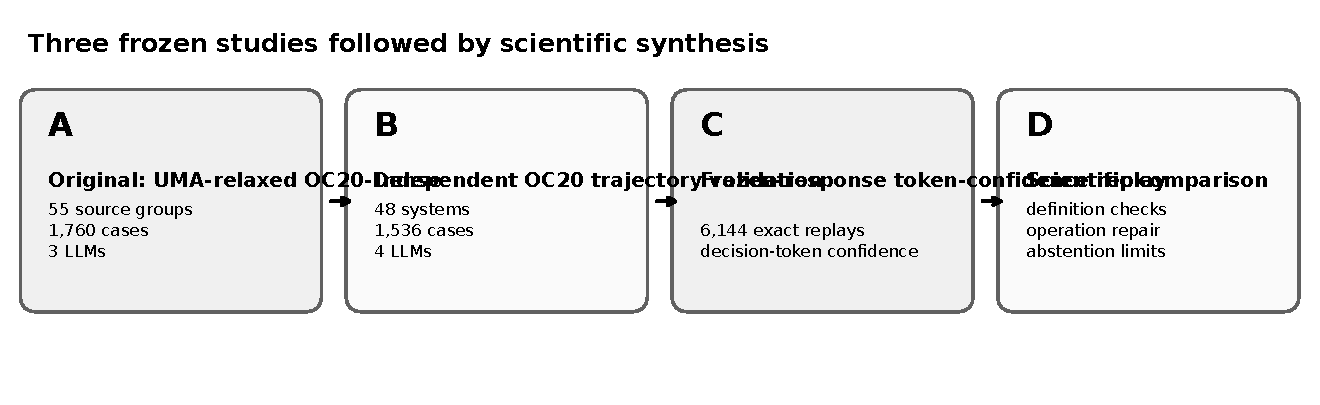
\includegraphics[width=\linewidth]{figure_01.pdf}
\captionof{figure}{One evidence-verification framework across UMA-relaxed and OC20 trajectory collections. The source-specific checks and confidence audit share physical definitions but retain their distinct scoring rules.}
\label{fig:workflow}
\end{minipage}
\end{center}

\subsection{RMSD definitions}

Root-mean-square deviation (RMSD) summarizes how far matched atoms differ between two structures. Its meaning depends on the selected atoms and the treatment of translation, rotation, and periodic boundaries. Atom correspondence was fixed throughout. For atom $i$, the displacement was
\begin{equation}
 \mathbf d_i=\operatorname{MIC}\!\left(\mathbf r_i^{(1)}-\mathbf r_i^{(0)}\right),
 \label{eq:displacement}
\end{equation}
Here, $i$ labels an atom, $\mathbf d_i$ is its displacement vector, and $\mathbf r_i^{(0)}$ and $\mathbf r_i^{(1)}$ are its initial and final positions. Periodic boundaries repeat the simulation cell. The function $\operatorname{MIC}$ selects the shortest equivalent displacement allowed by that cell. It was applied independently to each atom. The mobile-atom RMSD, $M$, and stored-frame adsorbate RMSD, $A$, were
\begin{equation}
 M=\left[\frac{1}{n_M}\sum_{i\in S_M}\|\mathbf d_i\|^2\right]^{1/2},
 \qquad
 A=\left[\frac{1}{n_A}\sum_{i\in S_A}\|\mathbf d_i\|^2\right]^{1/2}.
 \label{eq:frame}
\end{equation}
Here, $S_M$ and $S_A$ are the mobile and adsorbate atom sets, and $n_M$ and $n_A$ are their atom counts. The symbol $\|\cdot\|$ denotes vector length. Every atom received equal weight. Neither quantity removes molecular translation or rotation.

Internal RMSD, $I$, was calculated after the connected adsorbate was unwrapped at each endpoint. Unwrapping joins an adsorbate split across periodic boundaries into one connected image. The internal RMSD was
\begin{equation}
 I=\min_{\mathbf R,\mathbf t}
 \left[\frac{1}{n_A}\sum_{i\in S_A}
 \left\|\mathbf R\widetilde{\mathbf r}_i^{(0)}+\mathbf t
       -\widetilde{\mathbf r}_i^{(1)}\right\|^2\right]^{1/2}.
 \label{eq:internal}
\end{equation}
The positions $\widetilde{\mathbf r}_i^{(0)}$ and $\widetilde{\mathbf r}_i^{(1)}$ are the unwrapped coordinates. Here $\mathbf R$ is a rotation matrix, $\mathbf t$ is a translation vector, and $\min$ means we choose the pair that gives the smallest RMSD. A proper Kabsch rotation was used, which allows rotation but excludes reflection.\cite{kabsch1978discussion} No minimum-image correction was applied after fitting. All three RMSDs are reported in angstroms (\AA).

Because $S_A$ is a strict subset of $S_M$, their shared displacement convention gives
\begin{equation}
 M\geq A\sqrt{\frac{n_A}{n_M}},
 \qquad
 A\leq M\sqrt{\frac{n_M}{n_A}}.
 \label{eq:bounds}
\end{equation}
The bounds follow because the remaining mobile atoms add a nonnegative sum of squared displacements. They require the same comparison, frame, atom correspondence, periodic treatment, and equal weights. They do not provide a general bound between $I$ and $A$, which use different periodic and alignment procedures.

\subsection{Claims, evidence, and checking}

Each source group supplied 16 base claims. Each claim appeared as structured data and a short report. The final benchmark therefore contained 1,760 variants. Six base claims tested direct values, including unit conversion. Eight tested missing values using the bounds in Eq.~\ref{eq:bounds}. The last two supplied only fixed-atom evidence for missing internal RMSD, or evidence from another comparison. Thresholds were 0.75 or 1.25 times the relevant value or bound. These factors defined test cases, rather than chemical tolerances.

A claim was \emph{supported} when every value allowed by the evidence satisfied its inclusive inequality. It was \emph{contradicted} when every allowed value violated it. Otherwise, it had \emph{insufficient evidence}. The benchmark contained 550 supported, 550 contradicted, and 660 insufficient-evidence variants. The first two groups formed the 1,100 \emph{answerable cases}.

A \emph{licensed proof} was defined as one evidence record and one mathematical operation permitted by that record's physical definition. Operations could read a value, derive a mobile RMSD lower bound, or derive an adsorbate RMSD upper bound. Every alternative licensed proof was accepted. Generic relations were included in every prompt; the test did not require models to recall the bounds. Bound arithmetic used decimal precision of 50 digits. Coordinates and numerical cell vectors were not provided.

Evidence identifiers were replaced by neutral aliases, and records were shuffled. Both presentations retained the same numerical facts and physical definitions. The report presentation also removed redundant metric identifiers and display names. Thus, this comparison changed more than prose style alone.

\subsection{Model selection and proof-verification protocol}

The three models were Qwen3-4B-Instruct-2507, Phi-4-mini-instruct, and SmolLM3-3B, called Qwen, Phi, and SmolLM below. Each received two independent requests per variant. The \emph{direct-answer request} returned a scientific verdict, evidence identifier, and operation. The \emph{evidence-selection request} returned only the identifier and operation. Models had to follow a fixed JSON response format. One enclosing code-block wrapper was allowed; extra prose, unknown identifiers, invalid fields, and truncated responses were rejected without repair.

The same evidence selection was processed by three checks. The \emph{arithmetic-only check} applied the selected operation. The \emph{comparison-ID check} also required the requested comparison, meaning the specified pair of structures. The \emph{full-definition check} additionally required compatible atom sets, frame, alignment, periodic treatment, weights, and operation. No check searched for replacement evidence. A failed selection produced a \emph{workflow rejection}, which received no credit as scientific insufficiency. A separate \emph{deterministic oracle}, a program that tries every public record and permitted operation, established the task's solvability. All inference used one NVIDIA L40S GPU per model on UNL Swan. Generation used greedy decoding, which selects the most probable next token. Two requests were processed at a time using bfloat16 numerical precision. Each request allowed at most 160 new tokens and 6,144 input tokens. Inputs were not truncated. SmolLM extended thinking was disabled.

Direct-answer accuracy was measured both by verdict alone and by \emph{proof-aware accuracy}. The latter required a licensed proof for decisive claims or a correct explicit insufficiency response for insufficient claims. Valid numerical coverage was
\begin{equation}
 C=100\,\frac{N_{\mathrm{licensed}}}{N_{\mathrm{answerable}}}\;\%,
 \label{eq:coverage}
\end{equation}
where $C$ is the percentage of answerable cases answered correctly with a licensed proof. The counts $N_{\mathrm{licensed}}$ and $N_{\mathrm{answerable}}$ denote those valid answers and all answerable cases, respectively. Here, $N_{\mathrm{answerable}}=1{,}100$. An \emph{invalid acceptance} had either a wrong verdict or an unlicensed proof, even when its verdict happened to be correct.

Qwen was chosen during development for the primary comparison: full-definition versus comparison-ID checking on identical selections. Phi, SmolLM, and the presentation and task-family analyses were secondary. All 10,560 first attempts were retained, including malformed and output-cap failures. Uncertainty was estimated by resampling the 55 complete source groups 1,000 times (seed 20261021). All variants and paired conditions from a group remained together. Reported 95\% intervals are percentile intervals with linear interpolation and no multiple-testing adjustment. The protocol was fixed before final model inference, after development and source review; it was not externally preregistered.

\subsection{OC20 trajectory source collection and independent checks}
\label{sec:external_methods}

The complementary OC20 source collection uses the published OC20 IS2RE/IS2RS \texttt{val\_ood\_both} relaxation trajectories rather than the UMA-relaxed OC20-Dense systems in the original study.\cite{chanussot2021open} The original OC20 trajectory archive was downloaded and checked against its published MD5 digest. Each selected system supplies the first and last \emph{stored DFT relaxation frames}; we do not assume that the last stored frame reached a particular force tolerance or is a reference adsorption minimum. Independent hash ordering and predefined geometry qualification admitted 48 unique systems among the first 49 examined. This is a purposive qualified sample, not a random sample or a 48/49 acceptance-rate estimate for all OC20 trajectories.

The external geometry rules retain atom identity, surface-cell equality, periodic flags, and stationary fixed-atom constraints. The same shared-frame mobile RMSD ($M$), shared-frame adsorbate RMSD ($A$), and rigid-aligned internal RMSD ($I$) definitions are used as in Eqs.~\ref{eq:frame}--\ref{eq:bounds}. Each physical source pair also supplies one explicitly synthetic comparison control; those controls are not DFT relaxations. Each of 48 source groups contributes 16 base cases, each shown as structured evidence and as a written report. This gives 1,536 questions: 480 supported, 480 contradicted, and 576 insufficient-evidence cases. All valid one-record proof witnesses were sealed before external model inference; only public questions and evidence were sent to the models.

The external models are Qwen3-4B-Instruct-2507, Phi-4-mini-instruct, SmolLM3-3B, and Qwen3-32B-AWQ (4-bit weights). The 32B model is from the Qwen family and uses a different inference and quantization configuration; differences are not a controlled effect of parameter count. GPU generation was greedy with a 160-token output cap and 6,144-token input cap. Source groups were kept together across shards. The strict external score requires unfenced single-evidence JSON and a licensed conclusive proof on answerable cases. A separate diagnostic removes only an \emph{outer} Markdown JSON code fence; the model's evidence identifier, operation, and verdict are unchanged. The frozen operation-only repair checks an alternative permitted operation \emph{for the model-selected evidence identifier}; it is an oracle-assisted diagnostic ceiling, not a deployable inference method. When the complete public evidence and rules are available, the rule-only oracle enumerates all allowed proofs without any LLM selection.

\subsection{Confidence replay and statistical analysis}
\label{sec:confidence_methods}

The 1,536 external requests were replayed for each model with token probabilities recorded. All 6,144 replays reproduced the corresponding original answers exactly. We define \emph{decision-token confidence} as the geometric mean of conditional token probabilities for the chosen evidence identifier and mathematical operation. This token likelihood is \emph{not} interpreted as $P(\text{proof is correct})$. Confidence availability requires an unambiguous evidence identifier and operation; 42 answerable Phi cases and 225 answerable SmolLM cases had missing decision scores. We report those missing values, instead of imputing confidence. AUROC measures whether higher scores rank valid conclusive proofs above invalid ones on the 960 answerable cases per model; cases with insufficient evidence are analyzed separately. Within-model selective accuracy is measured by retaining the top 10\% of eligible answers. Uncertainty is descriptive, obtained by resampling complete OC20 source groups (48 clusters). These confidence outcomes are retrospective: the external correctness results had already been inspected, so no new untouched calibration or deployment threshold is claimed.
\subsection{External OC20 trajectory benchmark and independent checks}
\label{sec:external_methods}

The supplementary Phase 4 source collection uses the published OC20 IS2RE/IS2RS \texttt{val\_ood\_both} relaxation trajectories rather than the UMA-relaxed OC20-Dense systems in the original study.\cite{chanussot2021open} The original OC20 trajectory archive was downloaded and checked against its published MD5 digest (\texttt{bc74b6474a13542cc56eaa97bd51adfc}); the source-file SHA256 digest is pinned in the archived source manifest. Each selected system supplies the first and last \emph{stored DFT relaxation frames}; we do not assume that the last stored frame reached a particular force tolerance or is a reference adsorption minimum. Independent hash ordering and predefined geometry qualification admitted 48 unique systems among the first 49 examined. This is a purposive qualified sample, not a random sample or a 48/49 acceptance-rate estimate for all OC20 trajectories.

The external geometry rules retain atom identity, surface-cell equality, periodic flags, and stationary fixed-atom constraints. The same shared-frame mobile RMSD ($M$), shared-frame adsorbate RMSD ($A$), and rigid-aligned internal RMSD ($I$) definitions are used as in Eqs.~\ref{eq:frame}--\ref{eq:bounds}. Each physical source pair also supplies one explicitly synthetic comparison control; those controls are not DFT relaxations. Each of 48 source groups contributes 16 base cases, each shown as structured evidence and as a written report. This gives 1,536 questions: 480 supported, 480 contradicted, and 576 insufficient-evidence cases. All valid one-record proof witnesses were sealed before external model inference; only public questions and evidence were sent to the models.

The external models are Qwen3-4B-Instruct-2507, Phi-4-mini-instruct, SmolLM3-3B, and Qwen3-32B-AWQ (4-bit weights). The 32B model is from the Qwen family and uses a different inference and quantization configuration; differences are not a controlled effect of parameter count. GPU generation was greedy with a 160-token output cap and 6,144-token input cap. Source groups were kept together across shards. The strict external score requires unfenced single-evidence JSON and a licensed conclusive proof on answerable cases. A separate diagnostic removes only an \emph{outer} Markdown JSON code fence; the model's evidence identifier, operation, and verdict are unchanged. The frozen operation-only repair checks an alternative permitted operation \emph{for the model-selected evidence identifier}; it is an oracle-assisted diagnostic ceiling, not a deployable inference method. When the complete public evidence and rules are available, the rule-only oracle enumerates all allowed proofs without any LLM selection.

\subsection{Confidence replay and statistical analysis}
\label{sec:confidence_methods}

The 1,536 external requests were replayed for each model with token probabilities recorded. All 6,144 replays reproduced the corresponding original answers exactly. We define \emph{decision-token confidence} as the geometric mean of conditional token probabilities for the chosen evidence identifier and mathematical operation. This token likelihood is \emph{not} interpreted as $P(\text{proof is correct})$. Confidence availability requires an unambiguous evidence identifier and operation; 42 answerable Phi cases and 225 answerable SmolLM cases had missing decision scores. We report those missing values, instead of imputing confidence. AUROC measures whether higher scores rank valid conclusive proofs above invalid ones on the 960 answerable cases per model; cases with insufficient evidence are analyzed separately. Within-model selective accuracy is measured by retaining the top 10\% of eligible answers. Uncertainty is descriptive, obtained by resampling complete OC20 source groups (48 clusters). These confidence outcomes are retrospective: the external correctness results had already been inspected, so no new untouched calibration or deployment threshold is claimed. Raw per-token log-probability vectors were not archived; the recorded span scores and extraction code are preserved.

\section{Results}
\label{sec:results}

\subsection{Comparison identity alone does not license an atomistic proof}
\label{sec:primary}

The primary controlled comparison asks whether a measurement from the correct structure pair is necessarily suitable evidence. It is not. For Qwen, the comparison-ID checker accepted 393 numerical answers, but 81 were invalid under the supplied proof rules. The full-definition checker accepted 312: all 312 had correct verdicts and licensed proofs (Fig.~\ref{fig:checks}). Of the 81 additionally rejected acceptances, 42 had incorrect verdicts; the other 39 had verdicts that happened to be correct but relied on an incompatible measurement or operation. The latter errors would be invisible if evaluation checked only the final label.

All three checkers acted on identical raw evidence selections. The additional exclusions therefore arise from requiring the selected atom set, reference frame, alignment, periodic handling, weighting, and mathematical relation to match the claim, not from a new language-model prediction or an additional evidence search. The 81 prevented invalid acceptances equal 4.60 percentage points of all 1,760 cases (95\% source-group bootstrap interval 3.58--5.57). Full checking lost none of the 312 licensed answers. Within this defined task, run identity is necessary for using a record about the requested comparison, but is insufficient to establish that the selected quantity proves the claim.

\begin{figure}[tbp]
  \centering
  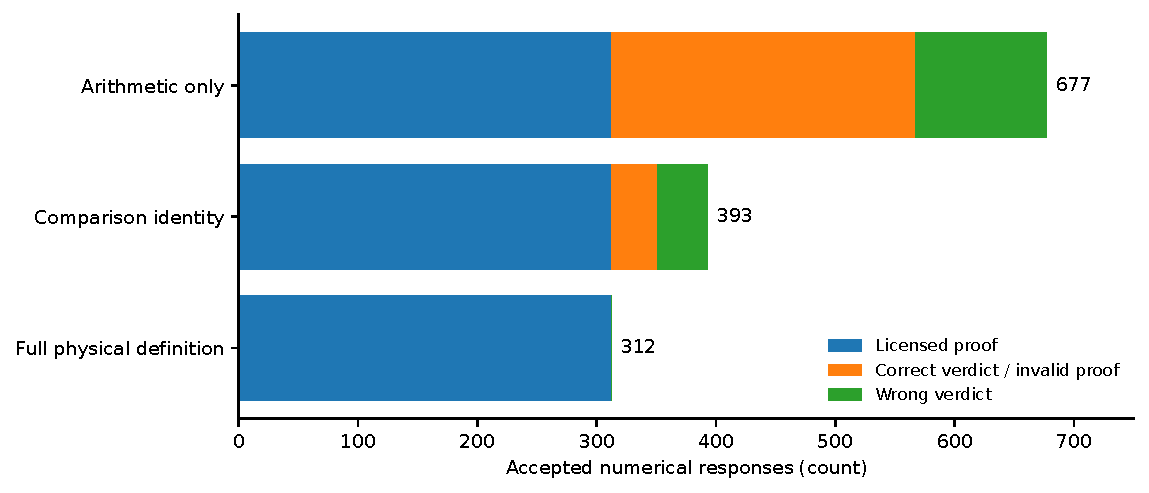
\includegraphics[width=\linewidth]{figure_02.pdf}
  \caption{Qwen numerical acceptances under arithmetic-only, comparison-ID, and full-definition checks on identical evidence selections. Stacked segments distinguish correctly licensed answers, wrong verdicts, and correct verdicts with unlicensed proofs.}
  \label{fig:checks}
\end{figure}

\subsection{Validation filters bad answers but does not recover missing proofs}
\label{sec:coverage_results}

The safety gain comes with a coverage cost. Of the 81 Qwen acceptances excluded only by full checking, 60 concerned answerable cases and 21 concerned insufficient-evidence cases. Thus, among the 1,100 answerable cases, accepted numerical answers decreased from 372 (33.82\%) under comparison-ID checking to 312 (28.36\%) under full checking, a decrease of 5.45 percentage points (95\% interval 4.09--6.91). The 312 retained answers are the same licensed answers in both conditions; the stricter checker supplies no replacement proof for the 60 newly rejected answerable cases.

The low coverage is not unique to Qwen. Full-definition valid numerical coverage was 121/1,100 (11.00\%) for Phi and 168/1,100 (15.27\%) for SmolLM (Supplementary Fig.~S2), against 312/1,100 for Qwen (95\% interval 25.73--31.00\%). Relative to comparison-ID checking, full checking prevented 245 additional invalid acceptances for Phi and 273 for SmolLM, again without rejecting any licensed answers. These are selective-filter results: correctness is assessed \emph{among accepted numerical answers}, not as 100\% overall task accuracy.

A deterministic oracle that enumerates permitted public-record proofs resolved all 1,760 cases, including all 1,100 answerable and all 660 insufficient-evidence cases. A valid proof therefore existed in the supplied packet for every answerable case, although the evaluated model--checker pipelines often failed to identify it. The oracle is a strong programmatic baseline for this constructed task and is not a trained language model.



\subsection{The physical definition changes what RMSD measures}
\label{sec:physical_results}

The coordinate evidence exhibits the underlying distinction. Across 55 source groups, stored-frame adsorbate RMSD exceeded aligned internal RMSD by more than a factor of ten in 16 groups; the median ratio was 3.27 (Supplementary Fig.~S1). Stored-frame RMSD retains positional and orientational displacement. In contrast, internal RMSD uses an unwrapped adsorbate followed by a proper rigid alignment, which removes overall translation and rotation.\cite{kabsch1978discussion} Equal distance units therefore do not make the quantities interchangeable.

The original system-by-system coordinates were not available in the frozen inputs used to regenerate figures; Supplementary Fig.~S1 accordingly displays only the documented aggregate statistics. This empirical comparison illustrates the motivation for testing physical definitions, but does not itself establish a universal inequality between stored-frame and internal RMSD. The shared-frame adsorbate and mobile-atom RMSDs, by contrast, admit explicit subset bounds because the adsorbate's equal-weight squared displacements are included in the mobile-atom sum (Eq.~\ref{eq:bounds}). The geometries are UMA-relaxed coordinates, not independent density-functional-theory validation of structural accuracy or adsorption energetics.



\subsection{Directly correct verdicts frequently lack valid proofs}
\label{sec:direct_results}

Direct-answer evaluation produces a second gap between an answer and its justification. Three-way verdict accuracy was 38.81\% for Qwen, 32.56\% for Phi, and 20.45\% for SmolLM. Requiring a valid proof on decisive claims, or a correct insufficiency response when appropriate, reduced proof-aware accuracy to 17.39\%, 23.01\%, and 3.75\%, respectively (Fig.~\ref{fig:direct}). The scores use all 1,760 variants, and proof-aware accuracy must not be confused with valid \emph{numerical} coverage of the 1,100 answerable cases.

Qwen gave numerical answers on 1,096 answerable cases, but only 255 combined a correct verdict with a licensed proof. It also gave numerical answers for 607 of 660 insufficient-evidence cases. Phi had 405 proof-aware successes in total, including 26 valid numerical answers and 379 correct insufficiency responses. These examples show how overall verdict scores can conceal the different outcomes of guessing a correct label, producing a valid proof, and correctly recognizing that the evidence cannot decide a claim.

The direct-answer and evidence-selection prompts were independent model requests. Therefore differences between direct performance and check-assisted selection performance cannot be interpreted as a causal effect of adding a checker. The matched causal isolation applies specifically to the three deterministic checkers processing the same selected records.

\begin{figure}[tbp]
  \centering
  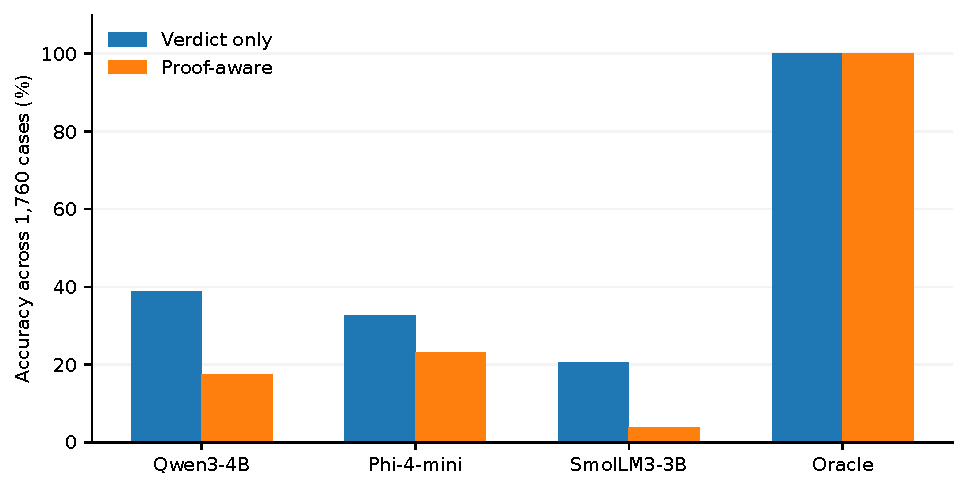
\includegraphics[width=\linewidth]{figure_03.pdf}
  \caption{Direct three-way verdict accuracy and proof-aware accuracy over 1,760 variants, compared with the deterministic oracle. Error bars indicate 95\% source-group bootstrap intervals.}
  \label{fig:direct}
\end{figure}

\subsection{Evidence presentation changes valid-answer coverage}
\label{sec:presentation_results}

The same underlying numerical facts did not yield equal success across presentations. Qwen's valid numerical coverage was 33.09\% on structured evidence versus 23.64\% on report-form evidence, a paired difference of 9.45 percentage points (95\% interval 4.73--13.82; Supplementary Fig.~S3). SmolLM showed a difference of 8.36 points (4.91--12.00). Phi's difference was $-0.18$ points ($-4.73$ to 3.82). Both presentations retained the relevant physical facts; however, the report rendering also omitted redundant metric names. Accordingly, the observed differences cannot be attributed to prose formatting alone.

The comparison is exploratory. It identifies a presentation-associated difference in selection success under the frozen prompts, but does not isolate the role of verbosity, naming cues, or an intrinsic change in physical reasoning.



\subsection{Selection failures depend on the permitted operation}
\label{sec:family_results}

Task-family performance was uneven (Supplementary Fig.~S4). Phi produced no licensed adsorbate upper-bound answer (0/220), while SmolLM produced no licensed mobile lower-bound answer (0/220). Qwen produced licensed answers in all four answerable families, with coverage ranging from 26.36\% for unit conversion to 34.55\% for mobile lower bounds. The oracle solved every family under the stated operation rules.

These outcomes identify which combinations of supplied records and permitted operations were difficult under this protocol. Bounds demand more than correct multiplication or comparison: the source and target atom sets, direction of the bound, and measurement convention must also match. These error patterns do not reveal the models' private reasoning or establish performance on general scientific problems.



\subsection{Four-model failure mechanisms persist on independently sourced OC20 trajectories}
\label{sec:external_results}

The external benchmark yielded 1,536 unique responses per model (6,144 total), without missing or duplicate request identifiers. Five SmolLM responses were truncated. A frozen public-evidence enumerator reconstructed all 1,536 sealed proof lists. We additionally audited the archived coordinates using independently written code: all 144 stored-frame mobile, adsorbate and fixed-atom RMSDs for 48 physical systems were reproduced to within $10^{-6}$~\AA; a separate bond-graph, periodic-unwrapping, and Kabsch implementation reproduced all 48 internal RMSDs, including the 33 multi-atom adsorbates. These independent calculations verify the archived numbers, but do not establish that the heuristic bond definitions are chemically complete. Figure~\ref{fig:external_geometry} illustrates the distinct physical meanings of the two external RMSD measures.

\begin{figure}[tbp]
  \centering
  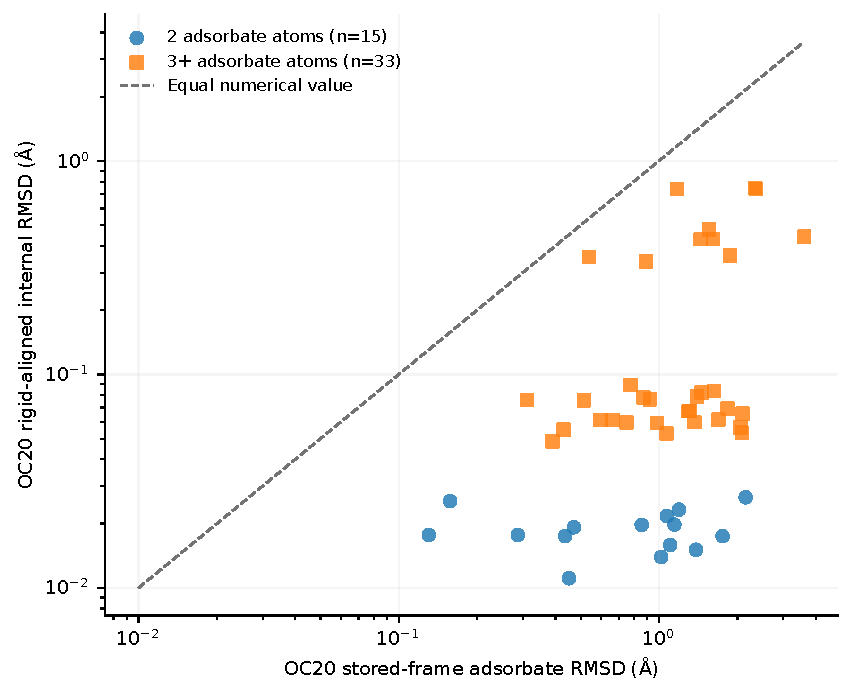
\includegraphics[width=0.75\linewidth]{figure_04.pdf}
  \caption{External OC20 physical measurement definitions for 48 independently sourced stored relaxation pairs. The stored-frame adsorbate RMSD and rigid-aligned internal RMSD need not agree because alignment removes rigid movement. Circles represent two-atom adsorbates; squares represent three or more atoms. This is the external set, not a reconstruction of the original 55 systems.}
  \label{fig:external_geometry}
\end{figure}


Table~\ref{tab:external} separates strict-format model performance from a diagnostic that removes only outer code fences. On 960 answerable questions, the fence-normalized 32B model produced 567 valid proofs (59.1\%), compared with 245 (25.5\%) for Qwen3-4B. The difference was 33.5 percentage points (95\% source-group bootstrap interval 30.4--36.7 points); this comparison is descriptive rather than a controlled scaling study. Strict-format success for Qwen3-32B was zero because every answer had a Markdown code fence. Its normalized result is therefore \emph{not} a strict-contract score. The operation-only diagnostic recovered additional proofs for every model, but still failed when a model selected the wrong endpoint or physical measurement.

\begin{table}[tbp]
\centering\small
\caption{External OC20 valid scientific proofs (960 answerable cases per model). Strict and fence-normalized model-only scores are distinct. The final column permits oracle-assisted operation replacement on an unchanged model-selected evidence identifier; it is not standalone model performance.}
\label{tab:external}
\begin{tabular}{lrrr}
\toprule
Model & Strict & Fence-normalized & After operation repair\\
\midrule
Qwen3-4B & 245 (25.5\%) & 245 (25.5\%) & 593 (61.8\%)\\
Phi-4-mini & 82 (8.5\%) & 97 (10.1\%) & 284 (29.6\%)\\
SmolLM3-3B & 1 (0.1\%) & 143 (14.9\%) & 260 (27.1\%)\\
Qwen3-32B-AWQ & 0 (0.0\%) & 567 (59.1\%) & 723 (75.3\%)\\
\bottomrule
\end{tabular}
\end{table}

\begin{figure}[tbp]
  \centering
  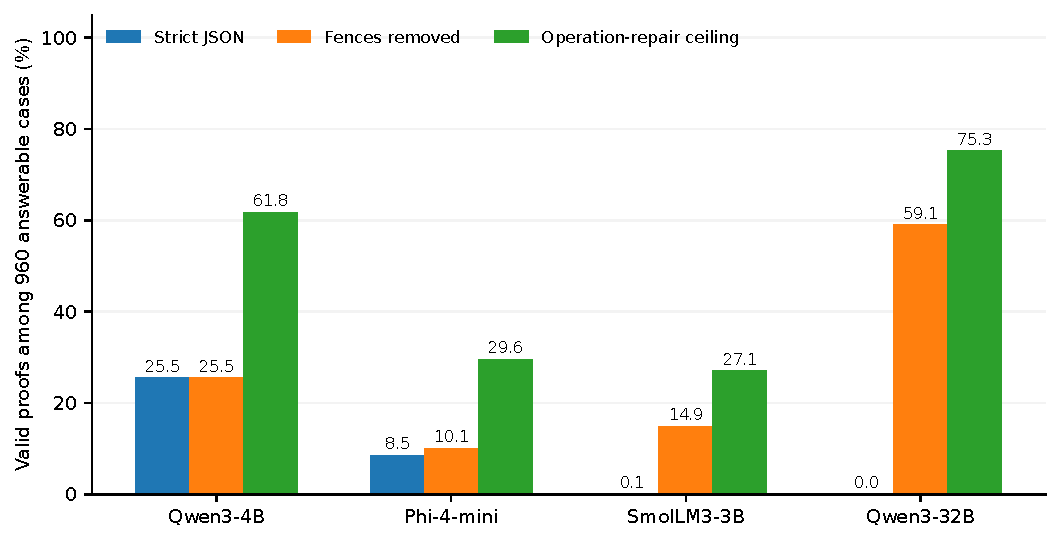
\includegraphics[width=\linewidth]{figure_05.pdf}
  \caption{Four-model proof validity on the external OC20 benchmark (960 answerable questions per model). Strict output parsing, outer-code-fence normalization, and oracle-assisted operation repair are distinct evaluations; the last two are diagnostic, not primary strict-contract results.}
  \label{fig:external_model_comparison}
\end{figure}

Among 960 answerable cases, Qwen3-32B produced 156 correct-evidence/wrong-operation selections, 131 wrong-endpoint choices, and 106 wrong or inconclusive measurement choices, in addition to 567 licensed proofs. It correctly used the evidence on 348 of 480 structured cases and 219 of 480 written-report cases; both presentations were correct for only 172 of 480 paired base cases. No model produced the required explicit scientific abstention on any of the 576 insufficient-evidence cases per model. A rejected proof was \emph{not} counted as a correct abstention. The presentation-specific error types are shown in Fig.~\ref{fig:external_error_types}.

\begin{figure}[tbp]
  \centering
  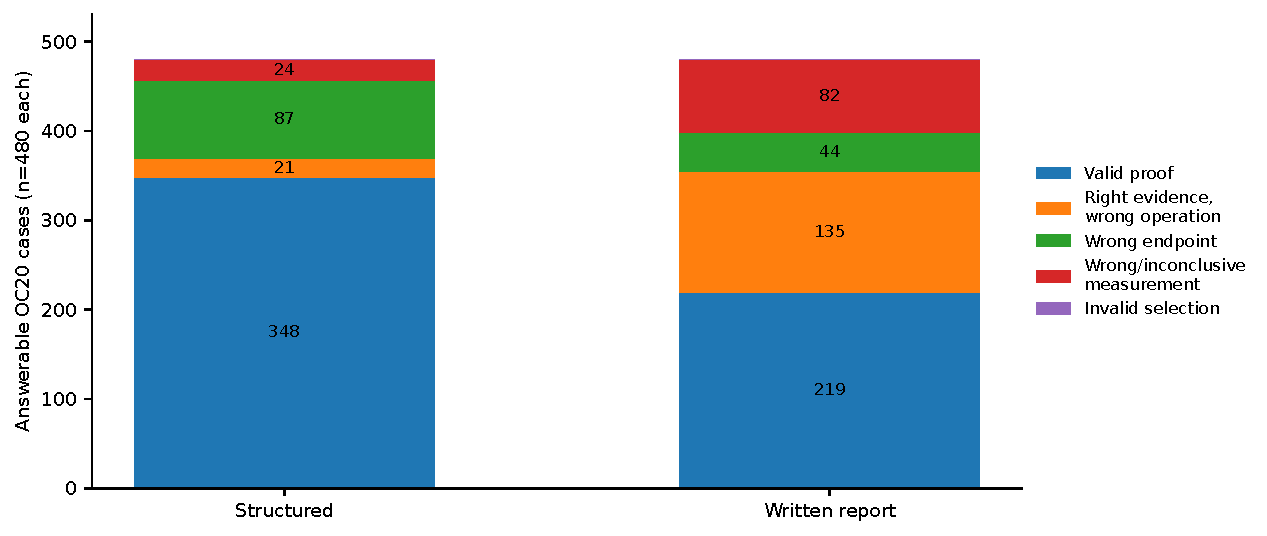
\includegraphics[width=0.88\linewidth]{figure_06.pdf}
  \caption{Qwen3-32B errors in structured and written OC20 presentations. Each presentation contains 480 answerable questions. A correct physical evidence ID with an incorrect operation is separated from a wrong endpoint comparison and a wrong physical measurement. Output code fences have been normalized for this diagnostic.}
  \label{fig:external_error_types}
\end{figure}


\subsection{High token likelihood is not a certificate of valid scientific evidence}
\label{sec:confidence_results}

The confidence replay recovered exactly the original 6,144 predictions. Decision-token scores ranked correct and incorrect answerable proofs better than chance for some models (Table~\ref{tab:confidence}). Qwen3-32B obtained AUROC 0.724 (95\% cluster-bootstrap interval 0.696--0.753), compared with 0.636 for Qwen3-4B, 0.552 for Phi, and 0.567 for SmolLM. Its most confident decile contained 90 valid and six invalid proofs among 96 eligible answers. However, among 601 Qwen3-32B answers with decision-token geometric mean above 0.99, 185 were scientifically invalid (30.8\%). This is not a formal miscalibration rate: token-generation likelihood has not been mapped to probability of scientific validity.

\begin{table}[tbp]
\centering\small
\caption{Confidence-based ranking on answerable OC20 cases. AUROC compares token confidence with licensed-proof correctness. Top-decile accuracy excludes missing decision-token scores. Confidence is not a calibrated probability of scientific truth.}
\label{tab:confidence}
\begin{tabular}{lrrr}
\toprule
Model & Score available & AUROC (95\% interval) & Top-decile valid\\
\midrule
Qwen3-4B & 960/960 & 0.636 (0.589--0.682) & 68/96\\
Phi-4-mini & 918/960 & 0.552 (0.484--0.626) & 18/92\\
SmolLM3-3B & 735/960 & 0.567 (0.507--0.620) & 22/74\\
Qwen3-32B-AWQ & 960/960 & 0.724 (0.696--0.753) & 90/96\\
\bottomrule
\end{tabular}
\end{table}

For Qwen3-32B, AUROC was 0.749 on structured cases and 0.647 on written reports, consistent with a presentation-dependent usefulness of confidence ranking. These are descriptive subgroup differences in correlated case pairs. The ROC results are restricted to answerable cases and cannot demonstrate recognition of insufficient evidence or reliable autonomous abstention. Figure~\ref{fig:confidence_revised} illustrates the ranking-versus-certification distinction.

\begin{figure}[tbp]
  \centering
  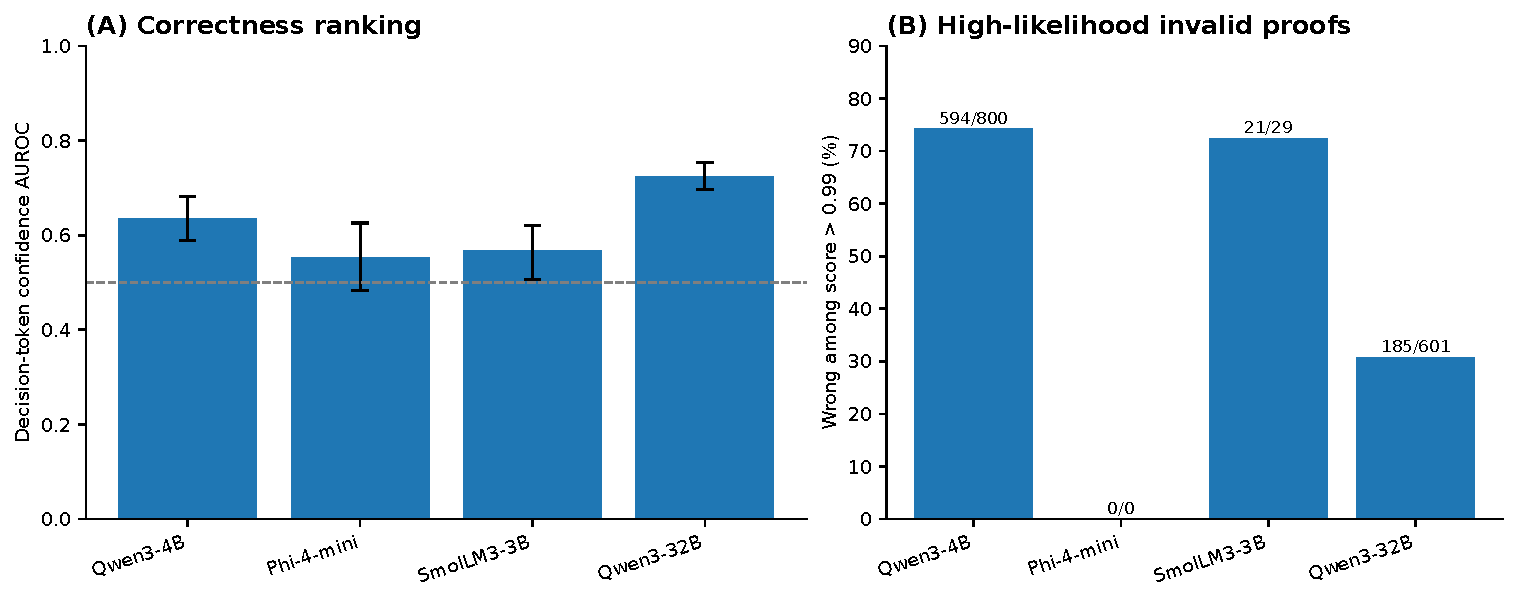
\includegraphics[width=\linewidth]{figure_07.pdf}
  \caption{Token confidence versus scientific correctness for the four models on answerable external cases. (A) Decision-token AUROC with 95\% source-group bootstrap intervals; 0.5 indicates chance-level ranking. (B) Fraction scientifically wrong among outputs with decision-token geometric mean above 0.99; Phi has no such outputs. These likelihoods are not calibrated probabilities of valid scientific proofs.}
  \label{fig:confidence_revised}
\end{figure}


\section{Discussion}
\label{sec:discussion}

\subsection{Scientific validity requires more than the right comparison}

The controlled checker comparison supports a specific conclusion: matching the source--endpoint comparison is not sufficient to establish that an atomistic number answers a physical question. A record can have the right comparison ID and an appropriate unit while describing different atoms, a different reference frame, or an unlicensed mathematical relation. These properties are independent of whether the final supported/contradicted verdict happens to be correct. The 39 Qwen cases with correct verdicts but invalid proofs make that distinction observable; a final-answer-only score would count them as successes even though the submitted evidence could not justify the answer.

This result fits within established research on scientific information selection and evidence-supported answers, including SciCUEval and ALCE.\cite{yu2026scicueval,gao2023enabling} GeoScope's more limited addition is a finite, physically specified RMSD setting in which the selected source, measurement definition, and mathematical operation can be checked against explicit proof rules. It does not establish that other scientific domains can be reduced to the same rules, or that a checker capable of handling every physical inference has been built.

\subsection{Verification and evidence selection remain separate problems}

Full checking improves the correctness of accepted numerical answers, but it is a filter, not a solution strategy. When an answerable Qwen selection fails validation, the checker does not examine alternate records to recover a permitted proof. As a result, the stricter criterion removes the invalid acceptances but leaves valid numerical coverage at 28.36\%. The deterministic oracle's success on every provided case shows that poor model-based selection, rather than an absence of task-defined evidence, is the bottleneck for these answerable cases. That comparison does not imply that all real atomistic questions have available, complete, or automatically checkable evidence.

This distinction matters for evaluation. High precision among the accepted answers can be obtained by making rejection more selective, even while the system resolves few scientific questions. Reporting proof validity without coverage would overstate practical capability; reporting verdict accuracy alone would hide unsupported conclusions. Direct answers, selections, workflow rejections, and genuine scientific insufficiency should therefore remain separate outcomes. Similarly, success of a deterministic oracle using explicit rules does not amount to improved language-model reasoning. A future system that searches for alternate licensed evidence would be a different method, to be evaluated separately from the present frozen checker comparison.

The presentation and operation results help locate the remaining selection problem, but not its cause. Report rendering removed redundant metric labels as well as changing the representation, and the response format required strict evidence--operation pairings within a 160-token output budget. Controlled presentation changes, alternative selection strategies, or more flexible output handling could improve usability, but the current data do not quantify such improvements. Tests of symbolic robustness provide useful context for these questions without supplying a direct explanation for GeoScope's observed differences.\cite{mirzadeh2025gsm}

\subsection{Limits of the conclusions and future tests}

The conclusions are bounded by the benchmark's construction. The 1,760 variants are correlated templates derived from 55 source groups, not 1,760 independent physical experiments. Uncertainty therefore resamples whole source groups. Those groups are disjoint from 20 development groups but remain within the same OC20-Dense domain; they are not a demonstrated test of unseen chemical families, independent DFT accuracy, or independence from UMA or language-model training data. Two adsorbate formulas account for 38 of the 55 accepted groups. All five excluded source systems had formula C$_2$H$_3$O$_2$, and 16 accepted groups retained descriptive chemical-contact flags. UMA convergence and geometric consistency do not by themselves establish chemically accurate adsorption structures, chemisorption, catalytic activity, or a global energy minimum.

The original matched-checker study evaluated three compact instruction models under one fixed greedy, no-extended-thinking inference protocol and its stated response format. The later OC20 experiment separately evaluated four models, including Qwen3-32B, with its distinct strict raw-JSON scoring contract and a fence-normalized diagnostic. All 10,560 first attempts were retained, including 261 SmolLM outputs truncated at the fixed token cap. The protocol was frozen after development and geometry-only review, before final model inference, but was not externally preregistered. The ability of full checking to accept no invalid proofs is conditional on this task's enumerated proof rules and is not evidence of 100\% overall accuracy or an unrestricted general guarantee. The results do not establish how larger models, longer inference, different prompts, or other scientific quantities would perform.

A substantive next step is to improve the \emph{selection} of compatible and conclusive evidence, not merely to make validation stricter. Candidate methods could enumerate admissible records before selecting an operation, perform a constrained search over proofs, or ask a model to revise a rejected selection using an explicit explanation of the physical mismatch. These are proposals, not experiments conducted here. Any new model, intervention, or scoring change should be evaluated using fresh source groups rather than tuned against the inspected final set, while retaining proof validity, valid numerical coverage, rejection rates, and scientific insufficiency as distinct outcomes.

\subsection{What independent scientific checking adds---and does not add}
\label{sec:external_discussion}

The combined experiments separate measurement choice from physical validity. The original matched-checker comparison establishes that strengthening physical-definition conditions excludes numerically plausible but unlicensed proofs without altering model outputs. The supplementary OC20 experiment demonstrates that the failure categories reappear on another source collection and persist with a larger open-weight model. The confidence replay adds a third distinction: a token can be highly probable while the measurement and operation that it describes are scientifically incompatible with the claim. Confidence may help prioritize manual review, especially for the 32B model, but cannot establish a valid proof or evidence sufficiency.

The rule-only enumerator resolves every benchmark case \emph{by construction}, because the structured packets include complete measurement definitions and the finite proof axioms. We therefore do not claim that the model--verifier approach surpasses deterministic-only checking. A model may be valuable for retrieving or interpreting unstructured evidence before checking, but the present experiments do not demonstrate that value in a controlled end-to-end comparison. The operation-repair numbers quantify an oracle-assisted recovery ceiling under fixed evidence identifiers; they must not be presented as an autonomously learned improvement.

The zero correct abstention rate under the frozen output contract is a limitation of this combination of models, prompts, and evaluation rules, not proof that the models cannot be taught to abstain. A future system should distinguish (i) a conclusive licensed proof, (ii) a complete evidence packet that licenses no conclusive proof, and (iii) unknown evidence completeness, conflicting definitions, or unreliable extraction requiring review. Confidence thresholds would need to be fitted on independent development systems, frozen, and tested prospectively for proof validity and abstention risk. The current retrospective ROC analysis is not such a calibration study.

Our new source audit checks the saved coordinate pairs against a second RMSD implementation, but does not establish independent chemical truth. In particular, the external data use saved DFT trajectory endpoints, not necessarily converged relaxed geometries. Synthetic distractors are labeled controls. The OC20 data may have appeared in language-model pretraining. The external questions are still controlled prompts using a restricted set of measurement definitions, and report rendering differs from structured evidence beyond a change in visual formatting. Independent internal RMSD recomputation agrees on all 48 systems, but expert assessment of the shared heuristic bond cutoff, broader periodic-boundary conventions, proof-policy adequacy, and raw token-log-probability reconstruction remain open audit items. The uploaded artifacts and manuscript draft are locally hash-frozen; the private GitHub repository, original figures, and Swan parent files have not been modified by this publication preparation.

\section{Conclusion}
\label{sec:conclusion}

GeoScope evaluates a single scientific requirement across two complementary atomic source collections: whether a language model's selected measurement and mathematical operation physically justify its conclusion. In the 55-system UMA collection, full-definition checking rejected 81 additional invalid Qwen selections relative to a comparison-ID check without excluding any of the 312 licensed proofs. The geometry analysis explains why this matters: whole-molecule displacement and internal deformation are distinct quantities even when calculated from the same structures. Correct final verdicts, therefore, cannot substitute for proof validity.

Using 48 OC20 DFT trajectory systems and four models, we found that the same class of evidence-selection failures persisted under a separate source and evaluation protocol. After removing only enclosing Markdown fences, the strongest tested model produced 567 valid proofs from 960 answerable questions (59.1\%). No model gave a qualifying abstention on its 576 insufficient-evidence questions. Model confidence could rank some valid proofs, but 185 of 601 Qwen3-32B selections with decision-token scores above 0.99 were still invalid. These tests establish complementary limits of evidence selection, operation choice, output formatting, and token likelihood; their differing scoring policies do not constitute identical replications or a controlled model-scaling experiment.

The central contribution is a physically defined, inspectable test of scientific justification rather than a new catalyst, a general scientific-reasoning solution, or a superior hybrid verifier. For autonomous materials research, it motivates keeping measurement definitions attached to claims and separating an invalid proof from genuinely missing evidence. Prospective evidence recovery, expert chemical review, and closed-loop validation are needed before improved materials-discovery outcomes can be claimed.

\section*{Supplementary Information}
A separately compiled Supplementary Information document provides the extended experiment protocols, original-study subgroup summaries, external-source audit, additional model comparisons, confidence analyses, reproducibility notes, and Figures S1--S11. Numerical results in the supplementary figures can be regenerated from the accompanying \texttt{publication\_figures} CSV and Python files. Independent chemical expert review remains outstanding.
\printbibliography
\end{document}
